% Author: Izaak Neutelings (June, 2018)
\documentclass[border=3pt,tikz]{standalone}
\usepackage{ifthen}
\usepackage{siunitx}
\usepackage{tikz}
\usetikzlibrary{hobby} % for ..
\usetikzlibrary{arrows.meta} % to control arrow size
\tikzset{>={Latex[length=4,width=4]}} % for LaTeX arrow head
\usetikzlibrary{calc,intersections,decorations.markings}
\usetikzlibrary{positioning,patterns,fadings}
\usepackage{siunitx}
\usepackage{xcolor} % for colored text

\colorlet{mylightblue}{blue!20}
\colorlet{myblue}{blue!50!black}
\colorlet{mydarkblue}{blue!30!black}
\colorlet{mylightred}{red!10}
\colorlet{myred}{red!50!black}
\colorlet{mydarkred}{red!60!black}
\colorlet{mydarkgreen}{green!30!black}
\definecolor{limegreen}{rgb}{0.2, 0.8, 0.2}

%\tikzstyle{midarr}=[decoration={markings,mark=at position 0.5 with {\arrow{stealth}}},postaction={decorate}]
\tikzset{
  midarr/.style={decoration={markings,mark=at position #1 with {\arrow{stealth}}},postaction={decorate}},
  midarr/.default=0.5
}
\def\tick#1#2{\draw[thick] (#1) ++ (#2:0.03*\ymax) --++ (#2-180:0.06*\ymax)}

\tikzset{
	mynode/.style n args={3}{
			postaction=decorate,
			decoration={
					markings,
					mark={at position #1 with \node[#2]{#3};}}}}

\begin{document}

% PV diagram - Maxwell construction
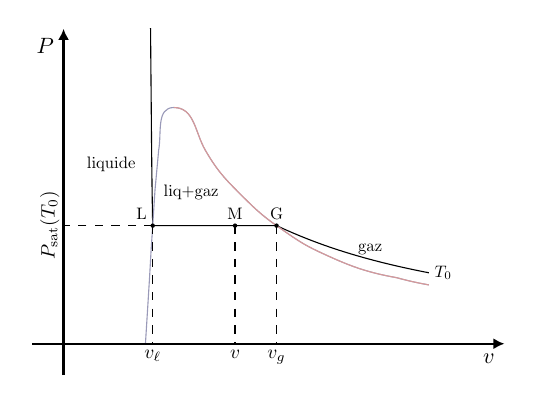
\begin{tikzpicture}
	\message{PV diagram - Maxwell construction^^J}
	\def\xmax{4}
	\def\ymax{4}
	\def\N{110}
	\def\s{0.6}
	\def\A{3}
	\def\isotherm#1#2{{ \A*(8*#2)/(3*#1-1) - 3*\A/(#1*#1) }}
	% reduced equation of state
	\coordinate (O) at (-0.2*\xmax,0);
	\coordinate (C) at (\s,\A);
	\coordinate (A) at (0.96*\xmax,\isotherm{0.96*\xmax/\s}{.85});
	\coordinate (D) at (0.08*\xmax,\isotherm{0.08*\xmax/\s}{.85});

	% LINE
	\foreach \i/\T/\pe in {0/.75/.28,1/.8/.39,2/.85/.5,3/.9/.65,4/.95/.82,5/1.0/1,6/1.1/1}{

			\begin{scope}
				\clip (-0.15*\xmax,0) rectangle (1.10*\xmax,\ymax);
				\ifthenelse{\i = 2}{
				% \draw[
				% green!80!white, path fading=east,
				% variable=\x,
				% domain=0.36:{.96*\xmax/\s},
				% range=0:1,samples=\N,smooth,name path=isotherm]
				% plot (\s*\x,\isotherm{\x}{\T});
				% \draw[
				% red!80!white, path fading=west,
				% variable=\x,
				% domain=0.36:{.96*\xmax/\s},
				% range=0:1,samples=\N,smooth]
				% plot (\s*\x,\isotherm{\x}{\T});
				\draw[
				black,
				variable=\x,
				domain=0.36:{.96*\xmax/\s},
				range=0:1,samples=\N,smooth,name path=isotherm]
				plot (\s*\x,\isotherm{\x}{\T})
				node[right,scale=0.6] {$T_0$};
				}{
				\path[mydarkblue,
				variable=\x,
				domain=0.36:{.96*\xmax/\s},
				range=0:1,samples=\N,smooth,name path=isotherm]
				plot (\s*\x,\isotherm{\x}{\T});
				}

				\ifthenelse{\i < 5}{ %\lengthtest{\pe pt < 1 pt}
					\path[name path={pe}] (0,\A*\pe) --++ ({.96*\xmax/\s},0);
					\path[name intersections={of=isotherm and pe,name=pe\i}];
				}

			\end{scope}
		}

	\begin{scope}
		\clip (0,0) rectangle (.96*\xmax,.96*\ymax);
		\fill[
			white,
			draw=mydarkblue!40,thin,use Hobby shortcut]
		(.06*\xmax,0) -- (pe0-1) -- (pe1-1) -- (pe2-1) -- (pe3-1) --
		(pe4-1) to[out=80,in=180]
		(C)
		to[out=0,in=120]
		(pe4-3) to[out=-60,in=135]
		(pe3-3) to[out=-45,in=145]
		(pe2-3) to[out=-35,in=155]
		(pe1-3) to[out=-25,in=170]
		(pe0-3) to[out=-15,in=170]
		(.97*\xmax,.185*\ymax) |- (0,0);
		\draw[mydarkred!40,thin,use Hobby shortcut]
		(C)
		to[out=0,in=120]
		(pe4-3) to[out=-60,in=135]
		(pe3-3) to[out=-45,in=145]
		(pe2-3) to[out=-35,in=155]
		(pe1-3) to[out=-25,in=170]
		(pe0-3) to[out=-15,in=170]
		(.97*\xmax,.185*\ymax) |- (0,0);
	\end{scope}
	\node[above left=35pt and 3pt, scale=0.6] at (pe0-1) {\strut liquide};
	\node[above left=5pt and 3pt,scale=0.6] at (pe0-3) {\strut gaz};
	\node[above right=25pt and 3pt,scale=0.6] at (pe0-1) {\strut liq+gaz};

	% MAXWELL CONSTRUCTION
	% \fill (C) circle (1pt) node[above, scale=.6] {C};
	\foreach \i in {2}{
			\draw[thin] (pe\i-1) -- (pe\i-3);
			\fill[black] (pe\i-3) circle (.8pt) node[above, scale=.6] {G};
			\fill[black] (pe\i-1) circle (.8pt) node[above left, scale=.6] {L};
			\fill[black]
			([shift={(-15pt,0)}]pe\i-3)
			coordinate (M)
			circle (.8pt) node[above, scale=.6] {M};
			% \fill[black] ([shift={(5pt,0)}]pe\i-1) circle (.8pt) node[above, scale=.6] {C};
		}
	% \fill (A) circle (.8pt) node[above, scale=.6] {A};
	% \fill (D) circle (.8pt) node[left, scale=.6] {D};

	% TICKS
	\draw[dashed] (pe2-3) -- (pe2-3|-O) node[below, scale=.7] {$v_g$};
	\draw[dashed] (pe2-1) -- (pe2-1|-O) node[below, scale=.7] {$v_{\ell}$};
	\draw[dashed] (M) -- (M|-O) node[below, scale=.7] {$v$};
	\draw[dashed] (pe2-1) -- (pe2-1-|O)
	node[left=5pt, rotate=90, anchor=center, scale=.7]
	{$P_{\rm sat}(T_0)$};

	% AXIS
	\draw[->,thick] (-0.2*\xmax,-0.1*\ymax) -- (-.2*\xmax,\ymax)
	node[anchor=north east,inner sep=4,scale=0.8] {$P$};
	\draw[->,thick] (-0.3*\xmax,0) -- (1.20*\xmax,0)
	node[anchor=north east,inner sep=4,scale=0.8] {$v$};

\end{tikzpicture}

\end{document}
